
\chapter{尤度比を使ったモデルとデータの比較}
\section{尤度比検定}
母数の個数が$k$個のモデル$M(\theta)$とする($\theta$は$k$次元ベクトル)。
モデル$M(\theta)$からサンプリングしたサンプルサイズ$n$の標本$x=(x_1,x_2,\cdots,x_n)$を得たとする。
この標本$X$から$\theta$のうち$r$個の母数に関する最尤推定量を$\bar{\theta}$得たとする。
$\bar{\theta}$のうち$k-r$個はモデル由来の母数であり、$r$個は標本から推定した母数である。
このことから、$\bar{\theta}$は自由度$r$の母数のベクトルと言う。

もとのモデル$M(\theta)$における標本$X$に対する尤度は、$L(\theta,x)$とする。
また、最尤モデル$M(\bar{\theta})$での尤度は、$L(\bar{\theta},x)$とする。
このとき、これら尤度の比がカイ二乗分布分布に従うことがわかっている\footnote{ただしいくらかの条件がある}。
つまり、
\begin{equation*}
    -2\log\lambda(X)\sim \chi^2_{k-r}
\end{equation*}
ただし、
\begin{equation*}
    \lambda(X) = \frac{L(\theta,x)}{L(\bar{\theta},x)} 
\end{equation*}
である。

\section{正規モデルにおける尤度比検定}

$\sigma^2_0$を設定した正規モデル$M(\mu_0;\sigma^2_0)$について考察する。
この正規モデルからサンプリングを行なった標本$X$とする。
標本から得た最尤正規モデルを$M(\bar{x};\sigma^2_0)$とする。
それぞれのモデル内での標本$X$の尤度を$L(\mu_0,X),L(\bar{x},X)$とする。
具体的な数式は、
\begin{align}
    L(\mu_0,X)=\frac{1}{\sqrt{2\pi\sigma^2}}\exp(-\frac{\sum(x_i-\mu_0)}{2\sigma^2})\\
    L(\bar{X},X)=\frac{1}{\sqrt{2\pi\sigma^2}}\exp(-\frac{\sum(x_i-\bar{X})}{2\sigma^2})\\
\end{align}
これらから$\lambda(X)$を計算すると、
\begin{align}
    -2\log\lambda(X) &= -2(-\frac{n}{2\sigma^2_0}(\bar{x}-\mu_0)^2) \\
    &= \frac{n}{\sigma^2_0}(\bar{x}-\mu_0)^2 \sim \chi^2_1 \\
\end{align}
である。

\subsubsection{数値実験}
モデルと同じ確率密度関数からサンプリングを行い、尤度比検定を行なってみる。

数値実験を行なってみる。具体的に、正規分布$N(170,5.8^2)$からサンプリングした標本1000個を集める。
標本から平均値を求め、これを最尤推定量とする(xbar)。
この最尤モデル$M(\mu;\sigma^2=5.8^2) $における標本の尤度を計算する(loglike2)。
同様に、モデル$M(170;\sigma^2=5.8^2)$における標本の尤度を計算する(loglike)。
以上から尤度比を計算し、それが$\chi^2_1$分布と一致することを確かめる。
以下がコードである。

\begin{lstlisting}
norm_ = norm(170,5.8)
data_ = norm.rvs(170,5.8,size=(1000,10))
xbar = np.average(data_,axis=1)
loglike_ = np.prod(norm_.pdf(data_),axis=1)
#loglike2_ = np.prod(norm(xbar,5.8).pdf(data_),axis=0)
#print(np.prod(norm(xbar,5.8).pdf(data_),axis=1),xbar)

loglike2_ = []
for item in data_:
    #print(item.shape)
    a = norm(np.average(item),5.8).pdf(item)
    loglike2_.append(np.prod(a))

y = -2*np.log(loglike_/loglike2_)
x = sorted(y)
y_ = np.arange(len(y))/len(x)
plt.plot(x,y_)
plt.plot(x,chi2.cdf(x,df=1))
plt.show()

\end{lstlisting}

$N(170,5.8^2)$と$N(175,5.8^2)$と言う2種類の密度関数からサンプリングを行いそれぞれ結果を図\ref{fig:loglikelihood_test_simulation_norm}(a)および(b)に示す。
図\ref{fig:loglikelihood_test_simulation_norm}(a)は、モデルとデータの分布が一致していることから、累積分布が$\chi^2_1$の累積分布にかなり近いことがわかる。
図\ref{fig:loglikelihood_test_simulation_norm}(b)は、モデルとデータが一致していない状況での結果を示している。尤度比の多くが右に移動しており、標本の多くが$\chi^2_1$において珍しいと判定されやすくなっている。


\begin{figure}
    \begin{center}
        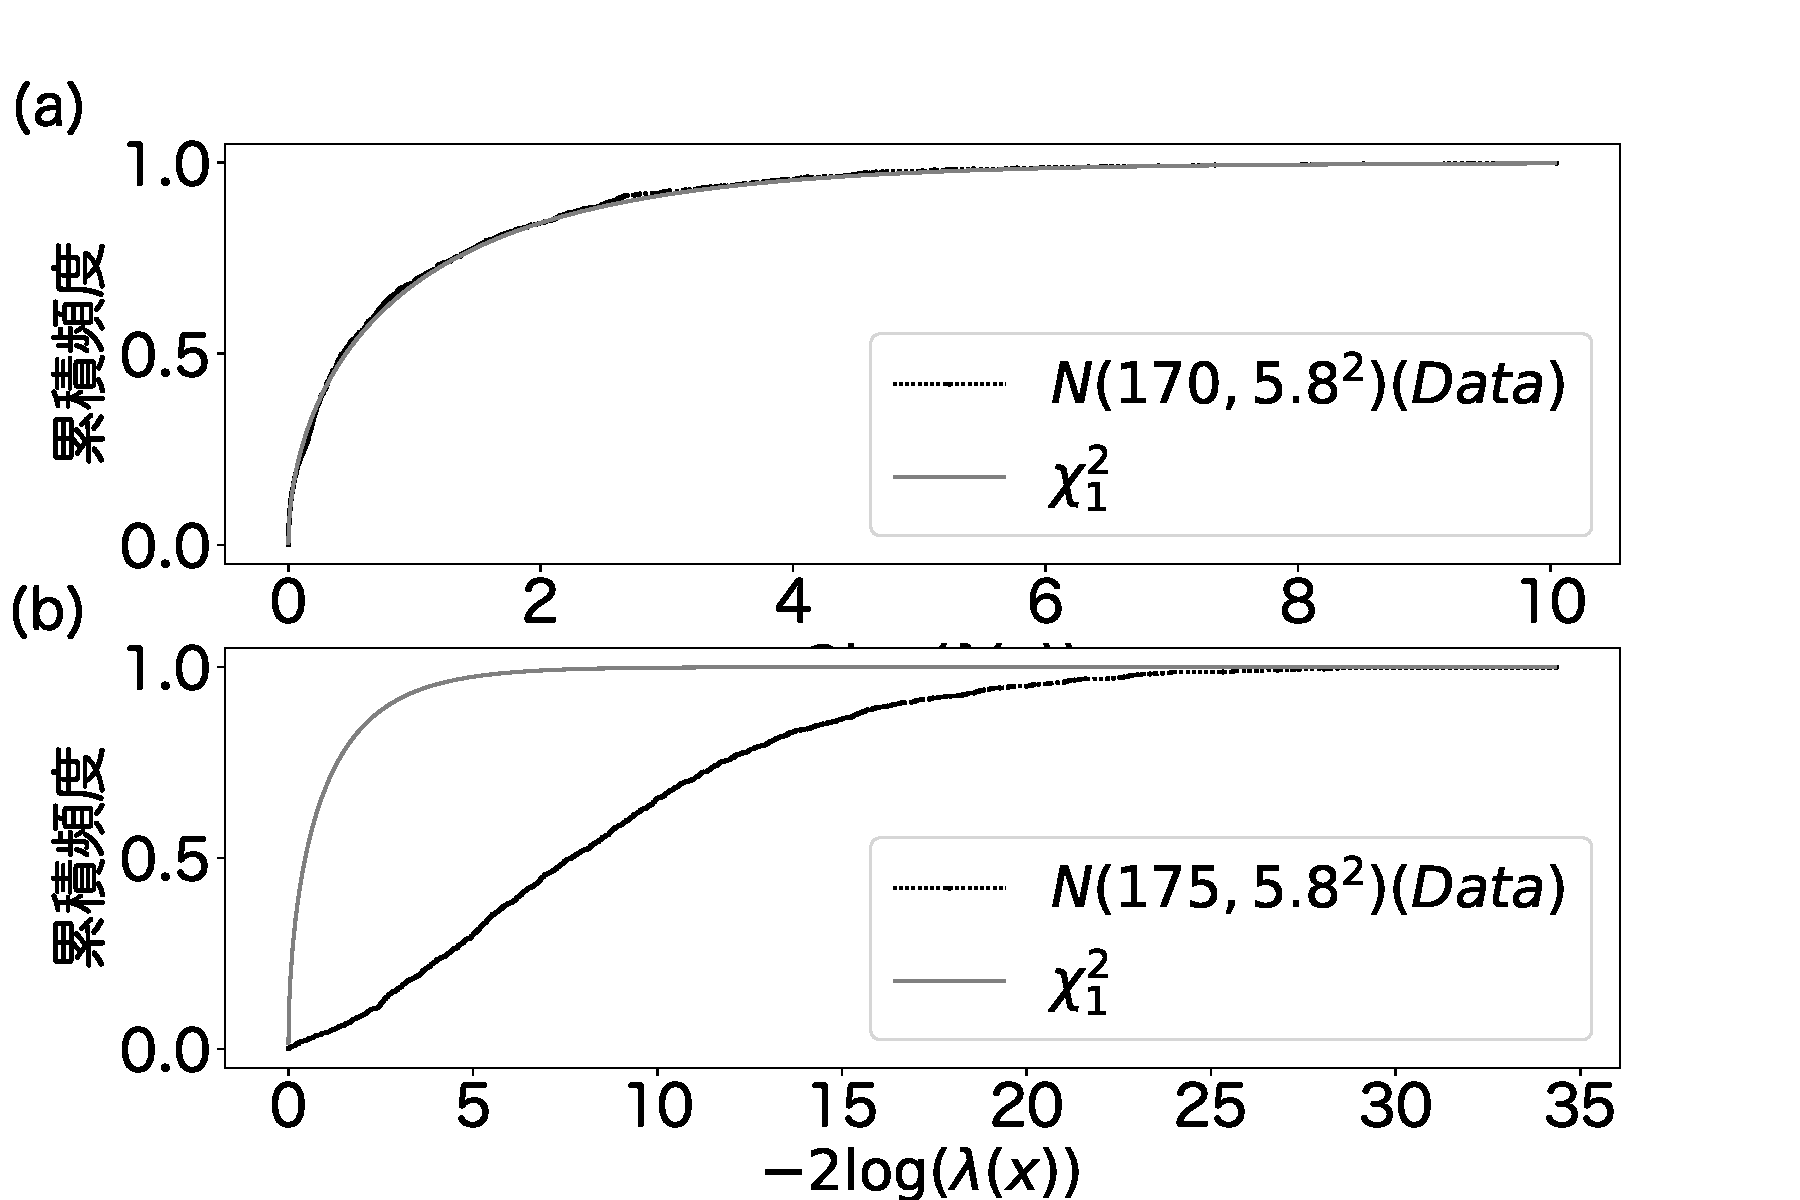
\includegraphics[width=15cm]{./image/04_/loglikeli_norm_test.pdf}
        \caption{対数尤度比の累積頻度。モデルは正規モデル$M(170;\sigma^2=5.8^2)$。(a)標本を$N(170,5.8^2)$からサンプリングした結果。(b)標本を$N(175,5.8^2)$からサンプリングした標本。}
        \label{fig:loglikelihood_test_simulation_norm}

      \end{center}
    \end{figure}

\subsection{データとモデルの乖離を検証する}
モデル上において、その標本を元にした最尤モデルにおける尤度比が$\chi^2_1$に従うことを示した。このことを元に、データをモデルによって予測可能かを調べる。手順は、
\begin{enumerate}
    \item 標本を$x$とする。
    \item モデル$M$における最尤推定量を計算する。
    \item モデル$M$および最尤モデル$M_{MLE}$における標本$x$に対する尤度を計算する
    \item 尤度比および$-2\log\lambda(x)$を計算し、$\chi^2_1$において珍しい値なのかを検証する。
\end{enumerate}
実際に、正規モデルにおいてこの手順をなぞってみる。
$M(\mu;\sigma^2)$における最尤モデルは、$M(\bar{x};\sigma^2)$である。
それぞれのモデルにおける尤度を計算し、$-2\log\lambda{x}$を計算すればよい。

